\documentclass{article}
\usepackage[margin = 0.5in]{geometry}
\usepackage[sc]{titlesec}
\usepackage{amsmath, pgfplots, array}
\pgfplotsset{compat = newest}
\setlength{\parindent}{0cm}
\pagestyle{empty}

\begin{document}

\subsubsection*{Graphing Parent Functions}

For each of the following fill out the table of values then plot the graph.

\begin{enumerate}   \setlength{\extrarowheight}{4pt}    \setlength{\itemsep}{0.5in}
    \item   \mbox{} \newline 
    \begin{minipage}{0.2\textwidth}
    \begin{tabular}{c|c}
        $\pmb{x}$ & $\pmb{f(x)=x}$ \\ \hline 
        $-5$ & \\ \hline 
        $-4$ & \\ \hline
        $-3$ & \\ \hline
        $-2$ & \\ \hline
        $-1$ & \\ \hline
        $0$ & \\ \hline
        $1$ & \\ \hline
        $2$ & \\ \hline
        $3$ & \\ \hline
        $4$ & \\ \hline
        $5$ & \\
    \end{tabular}
    \end{minipage}
    \begin{minipage}{0.5\textwidth}
    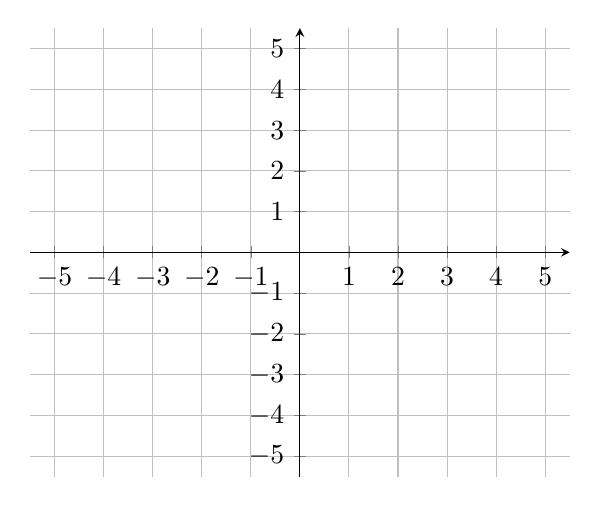
\begin{tikzpicture}
    \begin{axis}
    [axis lines = middle, xmin = -5.5, xmax = 5.5, ymin = -5.5, ymax = 5.5, xtick distance = 1, ytick distance = 1, grid]
    \end{axis}
    \end{tikzpicture}
    \end{minipage}
    
    \item   \mbox{} \newline 
    \begin{minipage}{0.2\textwidth}
    \begin{tabular}{c|c}
        $\pmb{x}$ & $\pmb{f(x)=|x|}$ \\ \hline 
        $-5$ & \\ \hline 
        $-4$ & \\ \hline
        $-3$ & \\ \hline
        $-2$ & \\ \hline
        $-1$ & \\ \hline
        $0$ & \\ \hline
        $1$ & \\ \hline
        $2$ & \\ \hline
        $3$ & \\ \hline
        $4$ & \\ \hline
        $5$ & \\
    \end{tabular}
    \end{minipage}
    \begin{minipage}{0.5\textwidth}
    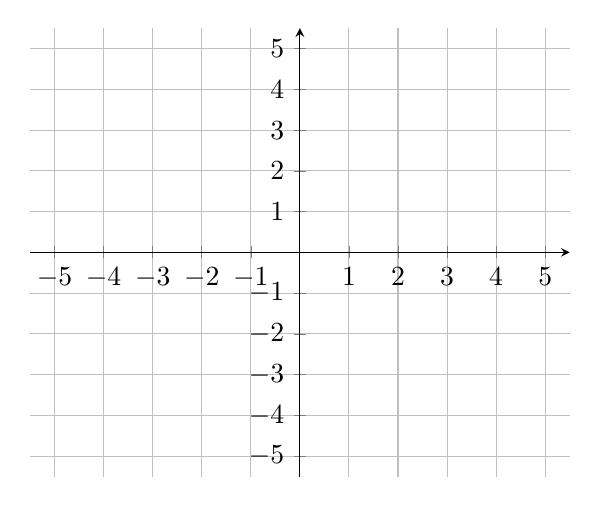
\begin{tikzpicture}
    \begin{axis}
    [axis lines = middle, xmin = -5.5, xmax = 5.5, ymin = -5.5, ymax = 5.5, xtick distance = 1, ytick distance = 1, grid]
    \end{axis}
    \end{tikzpicture}
    \end{minipage}
    
\item   \mbox{} \newline 
    \begin{minipage}{0.2\textwidth}
    \begin{tabular}{c|c}
        $\pmb{x}$ & $\pmb{f(x)=x^2}$ \\ \hline 
        $-4$ & \\ \hline
        $-3$ & \\ \hline
        $-2$ & \\ \hline
        $-1$ & \\ \hline
        $0$ & \\ \hline
        $1$ & \\ \hline
        $2$ & \\ \hline
        $3$ & \\ \hline
        $4$ & \\ 
    \end{tabular}
    \end{minipage}
    \begin{minipage}{0.5\textwidth}
    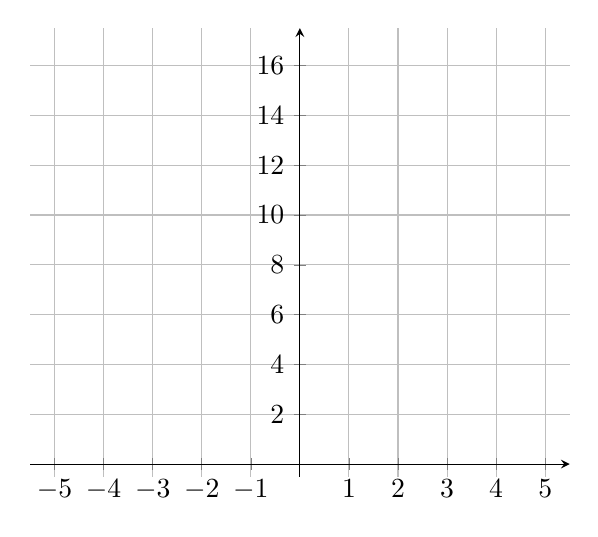
\begin{tikzpicture}
    \begin{axis}
    [axis lines = middle, xmin = -5.5, xmax = 5.5, ymin = -0.5, ymax = 17.5, xtick distance = 1, ytick distance = 2, grid]
    \end{axis}
    \end{tikzpicture}
    \end{minipage}
    
\item   \mbox{} \newline 
    \begin{minipage}{0.2\textwidth}
    \begin{tabular}{c|c}
        $\pmb{x}$ & $\pmb{f(x)=\sqrt{x}}$ \\ \hline 
        $0$ & \\ \hline
        $1$ & \\ \hline
        $2$ & \\ \hline
        $3$ & \\ \hline
        $4$ & \\ \hline 
        $5$ & \\ \hline 
        $6$ & \\ \hline 
        $7$ & \\ \hline 
        $8$ & \\ \hline 
        $9$ & \\ \hline 
    \end{tabular}
    \end{minipage}
    \begin{minipage}{0.5\textwidth}
    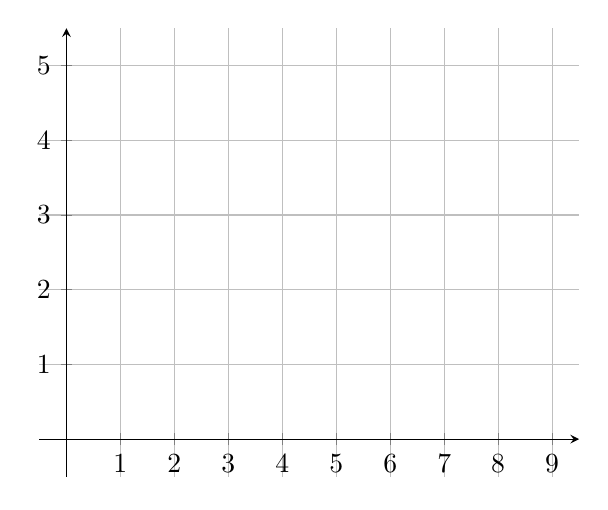
\begin{tikzpicture}
    \begin{axis}
    [axis lines = middle, xmin = -0.5, xmax = 9.5, ymin = -0.5, ymax = 5.5, xtick distance = 1, ytick distance = 1, grid]
    \end{axis}
    \end{tikzpicture}
    \end{minipage}
    
    \item   \mbox{} \newline 
    \begin{minipage}{0.2\textwidth}
    \begin{tabular}{c|c}
        $\pmb{x}$ & $\pmb{f(x)=\frac{1}{x}}$ \\ \hline 
        $-5$ & \\ \hline 
        $-4$ & \\ \hline
        $-3$ & \\ \hline
        $-2$ & \\ \hline
        $-1$ & \\ \hline
        $0$ & n/a \\ \hline
        $1$ & \\ \hline
        $2$ & \\ \hline
        $3$ & \\ \hline
        $4$ & \\ \hline
        $5$ & \\
    \end{tabular}
    \end{minipage}
    \begin{minipage}{0.5\textwidth}
    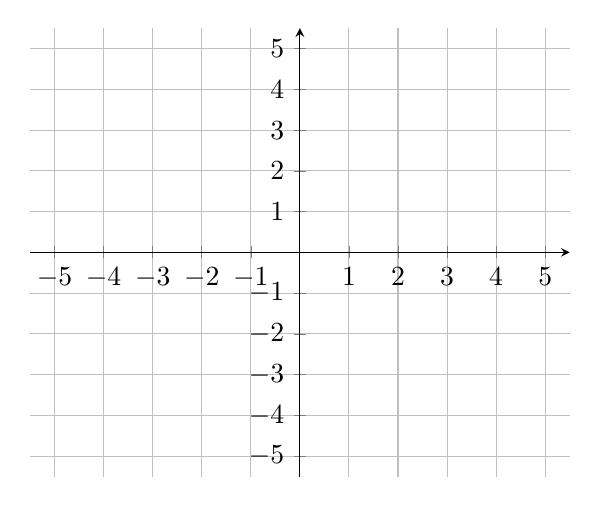
\begin{tikzpicture}
    \begin{axis}
    [axis lines = middle, xmin = -5.5, xmax = 5.5, ymin = -5.5, ymax = 5.5, xtick distance = 1, ytick distance = 1, grid]
    \end{axis}
    \end{tikzpicture}
    \end{minipage}
    
    % \item   \mbox{} \newline 
    % \begin{minipage}{0.2\textwidth}
    % \begin{tabular}{c|c}
    %     $\pmb{x}$ & $\pmb{f(x)=x^3}$ \\ \hline 
    %     $-3$ & \\ \hline
    %     $-2$ & \\ \hline
    %     $-1$ & \\ \hline
    %     $0$ & \\ \hline
    %     $1$ & \\ \hline
    %     $2$ & \\ \hline
    %     $3$ & \\ \hline
    % \end{tabular}
    % \end{minipage}
    % \begin{minipage}{0.5\textwidth}
    % \begin{tikzpicture}
    % \begin{axis}
    % [axis lines = middle, xmin = -3.5, xmax = 3.5, ymin = -27.5, ymax = 27.5, xtick distance = 1, ytick distance = 4, grid]
    % \end{axis}
    % \end{tikzpicture}
    % \end{minipage}
    
\end{enumerate}
\end{document}
